\begin{frame}
  \frametitle{Hybrid $S_N$-Diffusion Method: Proposed Work}
  \begin{block}{\textbf{Development of a Hybrid $S_N$-Diffusion Method for Control Rod Modeling}}
    \textbf{Sub-objectives}
    \begin{enumerate}
      \item Develop a robust submethod for resolving SVDCs near flux peaks and troughs
      \item Implement and extend the hybrid method for 2-D and 3-D reactor modeling in Moltres
      \item Investigate and rectify potential rod cusping errors
      \item Verify the hybrid method against reference OpenMC calculations
      \item Characterize the computational performance of the hybrid method
    \end{enumerate}
  \end{block}
\end{frame}

\begin{frame}
  \frametitle{Hybrid $S_N$-Diffusion Method: Proposed Work}
  \textbf{Sub-objective 1: Develop a robust submethod for resolving SVDCs near flux peaks and
  troughs}
  \vspace{.3cm}

  The existing formulation for SVDCs are undefined at flux peaks and troughs:
  \begin{align}
    D^s_g(x) &= -J^{tr}_g(x)\bigg/\frac{d\phi^{tr}_g(x)}{dx} \nonumber
  \end{align}
  I will explore alternative formulations to avoid division by the flux gradient. For instance,
  Tomatis \& Dall'Osso \cite{tomatis_application_2011} developed the following formulation for
  additive corrections:
  \begin{align}
    \delta D(x_{i+1/2},E) =& -\delta J(x_{i+1/2},E) \frac{(\Delta x_{i+1}+\Delta x_i)/2}{
    \phi(x_{i+1},E)-\phi(x_i,E)}
    \shortintertext{where}
    x_i =& \mbox{ $i$-th spatial interval,} \nonumber \\
    \delta J(x,E) =& J_{tr}(x,E) - J_D(x,E), \nonumber \\
    \Delta x_i =& \mbox{ size of $i$-th spatial interval.} \nonumber
  \end{align}
\end{frame}

\begin{frame}
  \frametitle{Hybrid $S_N$-Diffusion Method: Proposed Work}
  \textbf{Sub-objective 2: Implement and extend the hybrid method for 2-D and 3-D reactor modeling
  in Moltres}
  \vspace{.3cm}

  This sub-objective involves four main tasks:
  \begin{itemize}
    \item Implement a $S_N$ solver in Moltres/MOOSE
    \item Implement a coupling framework between the $S_N$ solver and the existing neutron
      diffusion solver
    \begin{itemize}
      \item Meshing of correction region
      \item Data transfers (e.g., flux, boundary conditions)
    \end{itemize}
    \item Determination of the correction region
      \begin{itemize}
        \item Develop a set of criteria for setting up the correction region
      \end{itemize}
    \item Autonomous determination of the buffer zone
  \end{itemize}
\end{frame}

\begin{frame}
  \frametitle{Hybrid $S_N$-Diffusion Method: Proposed Work}
  \textbf{Sub-objective 3: Investigate and rectify potential rod cusping errors}
  \vspace{.3cm}
  \begin{columns}
    \column[t]{6.5cm}
    Rod cusping occurs when the control rod boundary does not align perfectly with the mesh element
    boundaries when modeling time-dependent control rod insertion/withdrawal.
    \vspace{.1cm}
  
    Potential solutions:
    \begin{itemize}
      \item Adaptive meshing
      \item Approximate flux-volume weighting of cross sections
      \item Projection-based cusping treatment \cite{schunert_control_2019}
      \begin{itemize}
        \item Projection of piecewise constant cross sections onto a set of Legendre polynomials
        \item Exact integration of the FEM weak form is achieved
      \end{itemize}
    \end{itemize}
    \column[t]{5.5cm}
    \begin{figure}
      \centering
      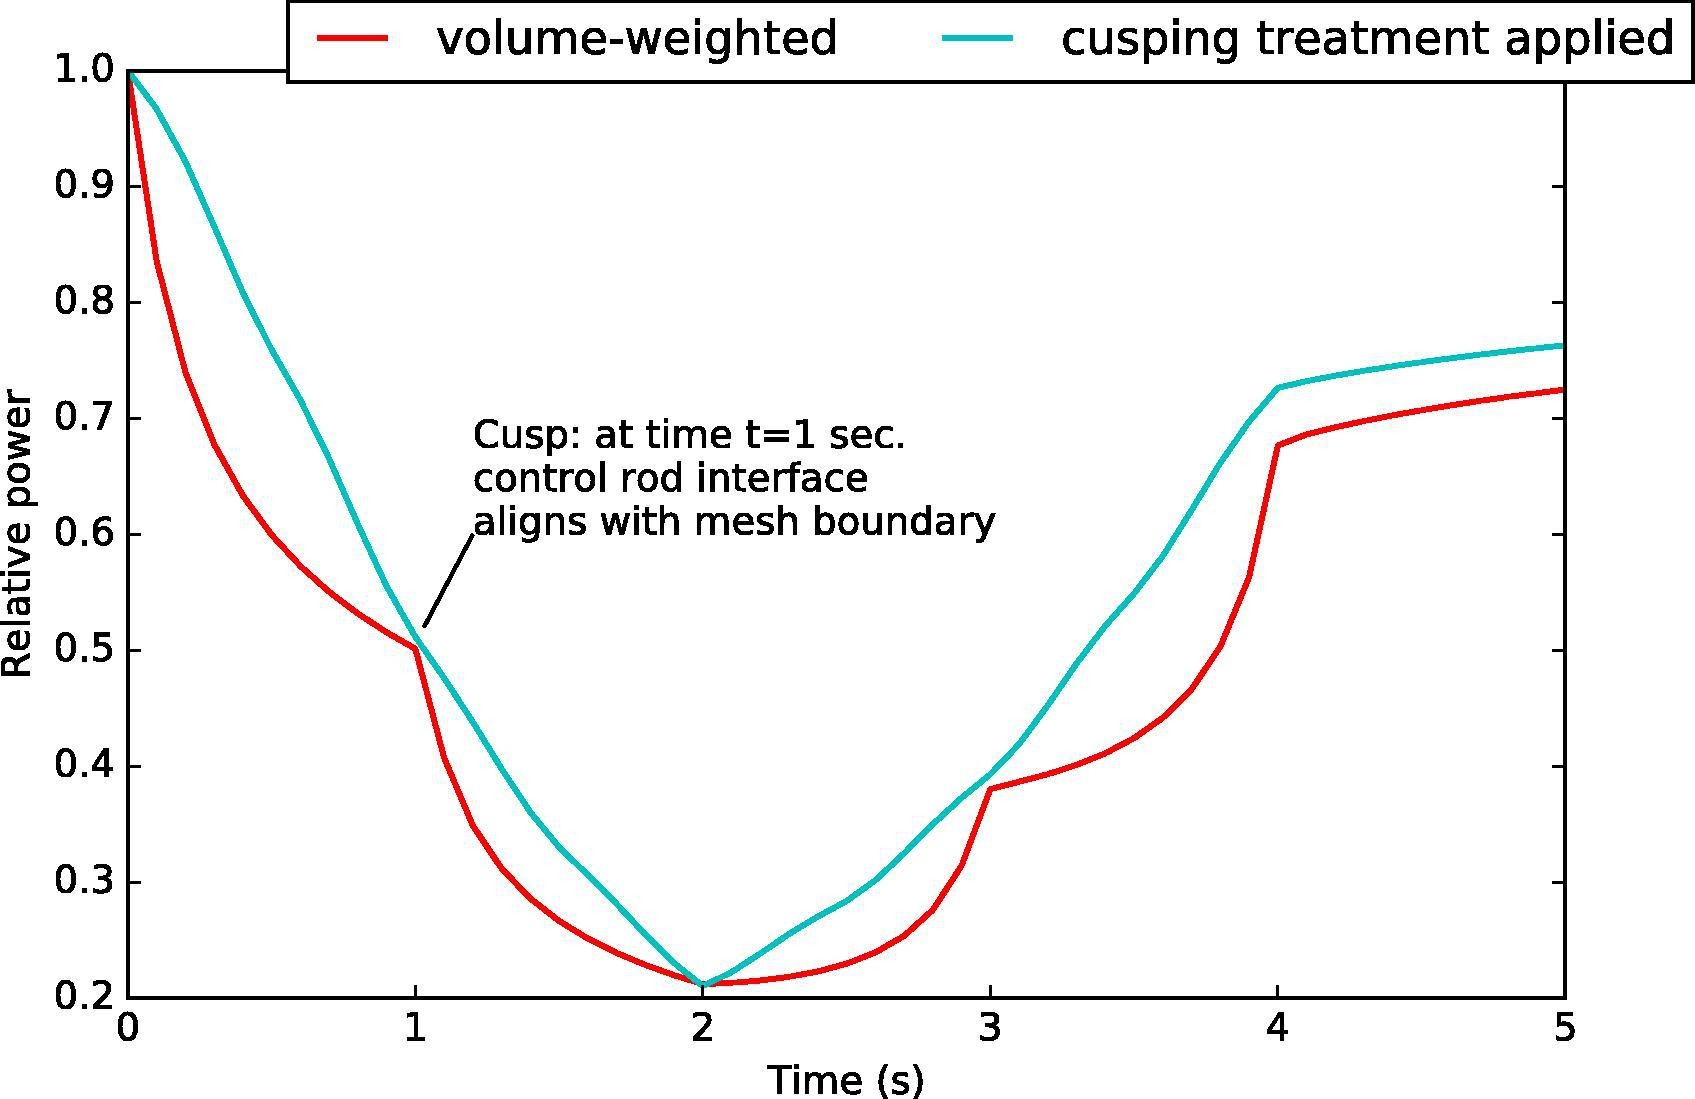
\includegraphics[width=.65\columnwidth]{images/cusping}
      \caption{Illustration of control rod cusping effect.}
      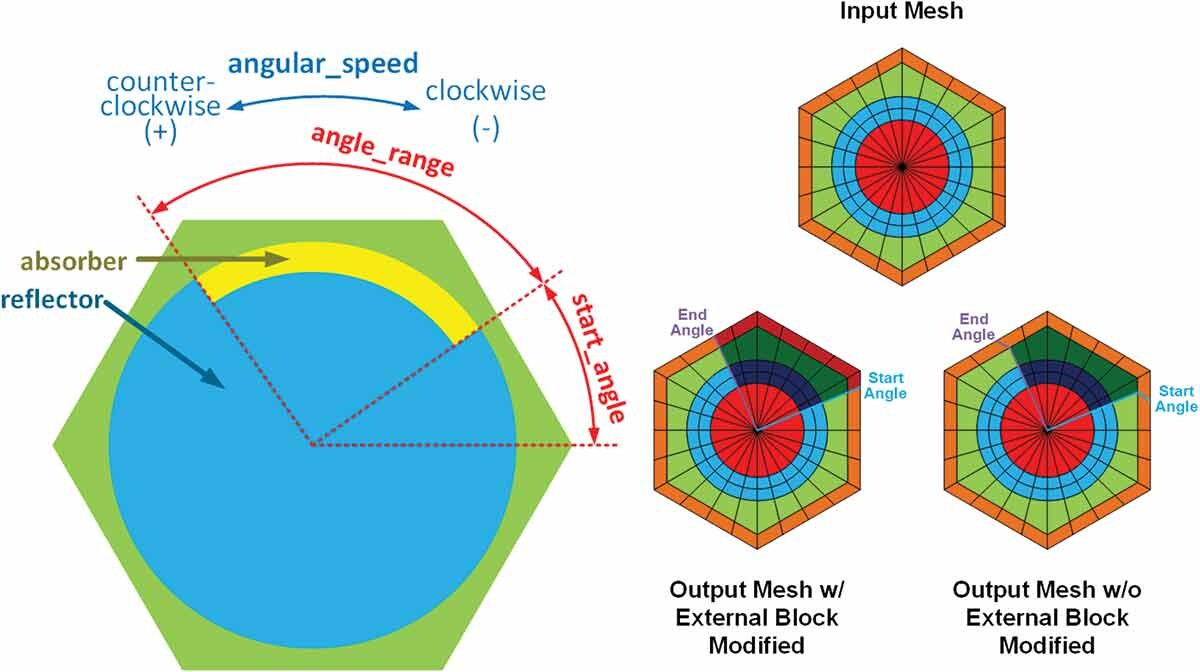
\includegraphics[width=.65\columnwidth]{images/control-drum}
      \caption{Adaptive meshing of a rotating control drum.}
    \end{figure}
  \end{columns}
\end{frame}

\begin{frame}
  \frametitle{Hybrid $S_N$-Diffusion Method: Proposed Work}
  \textbf{Sub-objective 4: Verify the hybrid method against reference OpenMC calculations}
  \vspace{.3cm}

  I will verify the hybrid method against reference OpenMC calculations of several toy problems,
  leading up to a 3-D model of the Molten Salt Reactor Experiment (MSRE). The verification study
  will include permutations of the following factors:
  \begin{itemize}
    \item 2-D and 3-D models
    \item Asymmetric control rod positions
    \item Static control rods at various levels of insertion
  \end{itemize}
  Stretch goal: Validate the hybrid method against the MSRE pump start-up and coast-down
  transients.
\end{frame}

\begin{frame}
  \frametitle{Hybrid $S_N$-Diffusion Method: Proposed Work}
  \textbf{Sub-objective 5: Characterize the computational performance of the hybrid method}
  \vspace{.3cm}

  The computational performance of the hybrid $S_N$-Diffusion method will be compared against the
  reference $S_N$ method. The hybrid method is expected to be faster due to:
  \begin{itemize}
    \item the small correction region size relative to the full reactor geometry
    \item faster convergence of SVDCs compared to neutron flux in $S_N$ calculations
  \end{itemize}
  Stretch goal: Explore the implementation of the hybrid method as a multischeme method,
  i.e., the $S_N$ and diffusion solvers run simultaneously.
\end{frame}
